% ===========================================================================
%  TikuOS — TikuKits DS: Hash Table for Embedded Systems
%  Beamer Presentation
% ===========================================================================
\documentclass[aspectratio=169, 10pt]{beamer}

% ---- Theme ----------------------------------------------------------------
\usetheme{Madrid}
\usecolortheme{whale}
\setbeamertemplate{navigation symbols}{}
\setbeamertemplate{footline}{%
  \leavevmode\hbox{%
    \begin{beamercolorbox}[wd=.33\paperwidth,ht=2.5ex,dp=1ex,center]{author in head/foot}%
      \usebeamerfont{author in head/foot}\insertshortauthor
    \end{beamercolorbox}%
    \begin{beamercolorbox}[wd=.34\paperwidth,ht=2.5ex,dp=1ex,center]{title in head/foot}%
      \usebeamerfont{title in head/foot}\insertshorttitle
    \end{beamercolorbox}%
    \begin{beamercolorbox}[wd=.33\paperwidth,ht=2.5ex,dp=1ex,right]{date in head/foot}%
      \usebeamerfont{date in head/foot}\insertshortdate{}\hspace*{2em}%
      \insertframenumber{}/\inserttotalframenumber\hspace*{2ex}
    \end{beamercolorbox}}%
  \vskip0pt%
}

% ---- Packages -------------------------------------------------------------
\usepackage{listings}
\usepackage{graphicx}
\usepackage{hyperref}
\usepackage{booktabs}
\usepackage{multirow}
\usepackage{tikz}
\usetikzlibrary{arrows.meta, positioning, shapes.geometric, calc,
                decorations.pathreplacing, fit}
\usepackage{amsmath}

% ---- Code listing style ---------------------------------------------------
\lstset{
  basicstyle=\ttfamily\scriptsize,
  keywordstyle=\color{blue}\bfseries,
  commentstyle=\color{gray},
  stringstyle=\color{red!70!black},
  showstringspaces=false,
  breaklines=true,
  frame=single,
  rulecolor=\color{black!30},
  backgroundcolor=\color{blue!3},
  tabsize=4,
}
\lstdefinestyle{cstyle}{
  language=C,
  morekeywords={uint8_t,uint16_t,uint32_t,int32_t,
                tiku_kits_ds_elem_t,tiku_kits_ds_htable_key_t,
                TIKU_KITS_DS_OK,TIKU_KITS_DS_ERR_NULL,
                TIKU_KITS_DS_ERR_FULL,TIKU_KITS_DS_ERR_PARAM,
                TIKU_KITS_DS_ERR_NOTFOUND,
                TIKU_KITS_DS_HTABLE_MAX_SIZE,
                TIKU_KITS_DS_HTABLE_EMPTY,
                TIKU_KITS_DS_HTABLE_OCCUPIED,
                TIKU_KITS_DS_HTABLE_DELETED,
                NULL,size_t},
}

% ---- Metadata -------------------------------------------------------------
\title[TikuKits DS]{TikuKits DS: Hash Table for Embedded Systems}
\subtitle{Simple. Ubiquitous. Intelligence, Everywhere.}
\author[Ambuj Varshney]{Ambuj Varshney \\ \texttt{ambuj@tiku-os.org}}
\date{\today}

% ===========================================================================
\begin{document}

% ---------------------------------------------------------------------------
\begin{frame}
\titlepage
\end{frame}

% ---------------------------------------------------------------------------
\begin{frame}{Outline}
\tableofcontents
\end{frame}

% ===========================================================================
\section{Motivation}
% ===========================================================================

\begin{frame}{Why a Hash Table on MCUs?}
\begin{columns}[T]
\begin{column}{0.48\textwidth}
\begin{block}{Embedded Use Cases}
\begin{itemize}
  \item \textbf{FRAM key-value store} --- persist configuration by key
  \item \textbf{Config lookup} --- map parameter IDs to values
  \item \textbf{String-to-enum mapping} --- command parsing
  \item \textbf{Device registry} --- map addresses to driver handles
\end{itemize}
\end{block}

\begin{block}{Constraints}
\begin{itemize}
  \item No heap allocation
  \item Limited RAM (2--8\,KB)
  \item Need $O(1)$ average-case lookup
  \item Must handle collisions gracefully
\end{itemize}
\end{block}
\end{column}

\begin{column}{0.48\textwidth}
\begin{center}
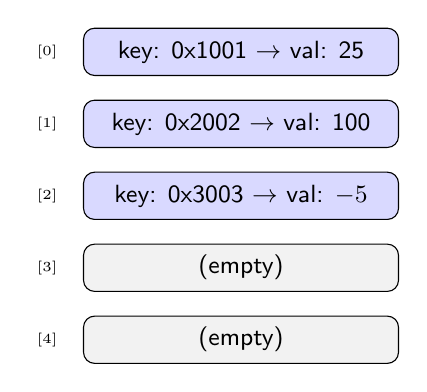
\begin{tikzpicture}[
    >=Stealth, node distance=0.5cm,
    kv/.style={draw, rounded corners, minimum height=0.6cm,
        minimum width=4cm, font=\small\sffamily}
  ]
  \node[kv, fill=blue!15] (k1) {key: 0x1001 $\rightarrow$ val: 25};
  \node[kv, fill=blue!15, below=0.3cm of k1] (k2)
    {key: 0x2002 $\rightarrow$ val: 100};
  \node[kv, fill=blue!15, below=0.3cm of k2] (k3)
    {key: 0x3003 $\rightarrow$ val: $-5$};
  \node[kv, fill=gray!10, below=0.3cm of k3] (k4) {(empty)};
  \node[kv, fill=gray!10, below=0.3cm of k4] (k5) {(empty)};

  \node[font=\tiny, left=0.2cm of k1] {[0]};
  \node[font=\tiny, left=0.2cm of k2] {[1]};
  \node[font=\tiny, left=0.2cm of k3] {[2]};
  \node[font=\tiny, left=0.2cm of k4] {[3]};
  \node[font=\tiny, left=0.2cm of k5] {[4]};
\end{tikzpicture}
\end{center}

\vspace{0.3em}
\begin{alertblock}{Design Goal}
Open-addressed hash table with \textbf{linear probing}, \textbf{FNV-1a} hashing,
and \textbf{tombstone deletion}. All storage statically allocated.
\end{alertblock}
\end{column}
\end{columns}
\end{frame}

% ===========================================================================
\section{Architecture}
% ===========================================================================

\begin{frame}{Open Addressing with Linear Probing}
\begin{columns}[T]
\begin{column}{0.48\textwidth}
\textbf{Open addressing:} All entries live in a single flat array.
No linked lists of buckets --- saves memory and cache misses.

\vspace{0.5em}
\textbf{Linear probing:} On collision, check the next slot, then
the next, wrapping around. Simple and cache-friendly.

\vspace{0.5em}
\textbf{Insert algorithm:}
\begin{enumerate}
  \item Compute \texttt{idx = hash(key) \% capacity}
  \item If slot is EMPTY or key matches: insert/update
  \item If slot is OCCUPIED with different key: try \texttt{idx+1}
  \item Wrap around if needed
\end{enumerate}

\vspace{0.3em}
\textbf{Lookup:} Same probe sequence. Stop at EMPTY (key not present)
or matching key (found). Skip DELETED slots during search.

\vspace{0.3em}
\begin{block}{Complexity}
Average case: $O(1)$ for put/get/remove.\\
Worst case: $O(n)$ when heavily loaded.
\end{block}
\end{column}

\begin{column}{0.48\textwidth}
\begin{center}
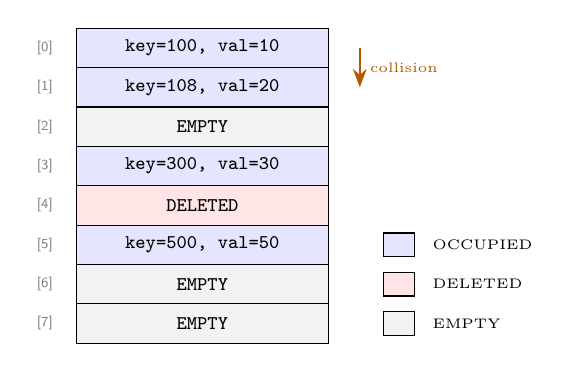
\begin{tikzpicture}[
    >=Stealth,
    slot/.style={draw, minimum width=3.2cm, minimum height=0.5cm,
                 font=\scriptsize\ttfamily},
    idx/.style={font=\tiny\sffamily, text=gray}
  ]
  % Array slots
  \node[slot, fill=blue!10] (s0) at (0, 0) {key=100, val=10};
  \node[slot, fill=blue!10] (s1) at (0, -0.5) {key=108, val=20};
  \node[slot, fill=gray!10] (s2) at (0, -1.0) {EMPTY};
  \node[slot, fill=blue!10] (s3) at (0, -1.5) {key=300, val=30};
  \node[slot, fill=red!10] (s4) at (0, -2.0) {DELETED};
  \node[slot, fill=blue!10] (s5) at (0, -2.5) {key=500, val=50};
  \node[slot, fill=gray!10] (s6) at (0, -3.0) {EMPTY};
  \node[slot, fill=gray!10] (s7) at (0, -3.5) {EMPTY};

  % Indices
  \foreach \i in {0,...,7} {
    \node[idx] at (-2.0, -\i*0.5) {[\i]};
  }

  % Collision arrow
  \draw[->, thick, orange!70!black] (2.0, 0) -- (2.0, -0.5)
    node[midway, right, font=\tiny] {collision};

  % Legend
  \node[font=\tiny, fill=blue!10, draw, minimum width=0.4cm,
        minimum height=0.3cm] at (2.5, -2.5) {};
  \node[font=\tiny, right] at (2.8, -2.5) {OCCUPIED};

  \node[font=\tiny, fill=red!10, draw, minimum width=0.4cm,
        minimum height=0.3cm] at (2.5, -3.0) {};
  \node[font=\tiny, right] at (2.8, -3.0) {DELETED};

  \node[font=\tiny, fill=gray!10, draw, minimum width=0.4cm,
        minimum height=0.3cm] at (2.5, -3.5) {};
  \node[font=\tiny, right] at (2.8, -3.5) {EMPTY};
\end{tikzpicture}
\end{center}
\end{column}
\end{columns}
\end{frame}

% ===========================================================================
\section{Data Structure}
% ===========================================================================

\begin{frame}[fragile]{The \texttt{tiku\_kits\_ds\_htable} Structures}
\begin{columns}[T]
\begin{column}{0.48\textwidth}
\begin{lstlisting}[style=cstyle,
  title={ds/htable/tiku\_kits\_ds\_htable.h}]
#define TIKU_KITS_DS_HTABLE_MAX_SIZE 16

#define TIKU_KITS_DS_HTABLE_EMPTY     0
#define TIKU_KITS_DS_HTABLE_OCCUPIED  1
#define TIKU_KITS_DS_HTABLE_DELETED   2

typedef uint32_t
    tiku_kits_ds_htable_key_t;

struct tiku_kits_ds_htable_entry {
    tiku_kits_ds_htable_key_t key;
    tiku_kits_ds_elem_t value;
    uint8_t state;
};

struct tiku_kits_ds_htable {
    struct tiku_kits_ds_htable_entry
        entries[
         TIKU_KITS_DS_HTABLE_MAX_SIZE];
    uint16_t capacity;
    uint16_t count;
};
\end{lstlisting}
\end{column}

\begin{column}{0.48\textwidth}
\textbf{Memory footprint} (default config):\\
Per entry: $4 + 4 + 1 = 9$ bytes\\
Total: $16 \times 9 + 2 + 2 = 148$ bytes\\
All statically allocated --- no heap.

\vspace{0.5em}
\begin{block}{Three-State Slots}
\begin{itemize}
  \item \textbf{EMPTY} (0) --- never used
  \item \textbf{OCCUPIED} (1) --- holds a live key-value pair
  \item \textbf{DELETED} (2) --- tombstone; was occupied, now removed
\end{itemize}
\end{block}

\vspace{0.3em}
\begin{alertblock}{Key Type}
Keys are \texttt{uint32\_t} --- suitable for address IDs,
CRC values, or hashed string identifiers.
Values use the shared \texttt{tiku\_kits\_ds\_elem\_t} type.
\end{alertblock}
\end{column}
\end{columns}
\end{frame}

% ===========================================================================
\section{API Reference}
% ===========================================================================

\begin{frame}[fragile]{Complete API}
\begin{table}
\centering
\small
\begin{tabular}{@{}lp{8cm}@{}}
\toprule
\textbf{Function} & \textbf{Description} \\
\midrule
\texttt{tiku\_kits\_ds\_htable\_init(ht, cap)}
  & Initialize with \texttt{cap} slots, all marked EMPTY \\
\midrule
\texttt{tiku\_kits\_ds\_htable\_put(ht, key, val)}
  & Insert new key-value pair or update existing key \\
\texttt{tiku\_kits\_ds\_htable\_get(ht, key, \&val)}
  & Look up key, return value or ERR\_NOTFOUND \\
\texttt{tiku\_kits\_ds\_htable\_remove(ht, key)}
  & Tombstone-delete a key (marks slot DELETED) \\
\midrule
\texttt{tiku\_kits\_ds\_htable\_contains(ht, key)}
  & Returns 1 if key exists, 0 otherwise \\
\texttt{tiku\_kits\_ds\_htable\_clear(ht)}
  & Mark all entries EMPTY, reset count \\
\texttt{tiku\_kits\_ds\_htable\_count(ht)}
  & Number of OCCUPIED entries \\
\bottomrule
\end{tabular}
\end{table}

\vspace{0.3em}
\begin{alertblock}{Put Semantics}
\texttt{put()} performs an \textbf{upsert}: if the key already exists, its value
is updated in place (count unchanged). If the key is new, a new entry is created.
\end{alertblock}
\end{frame}

% ===========================================================================
\section{FNV-1a Hash Function}
% ===========================================================================

\begin{frame}[fragile]{FNV-1a: Hashing uint32\_t Keys}
\begin{columns}[T]
\begin{column}{0.48\textwidth}
\begin{lstlisting}[style=cstyle,
  title={FNV-1a hash implementation}]
static uint16_t hash_fnv1a(
    tiku_kits_ds_htable_key_t key,
    uint16_t capacity)
{
    uint32_t h = 2166136261u;
    uint8_t i;

    for (i = 0; i < 4; i++) {
        h ^= (key >> (i * 8)) & 0xFF;
        h *= 16777619u;
    }
    return (uint16_t)(h % capacity);
}
\end{lstlisting}

\vspace{0.3em}
\textbf{Constants:}\\
Offset basis: \texttt{2166136261} (FNV-1a 32-bit)\\
Prime: \texttt{16777619} (FNV-1a 32-bit)
\end{column}

\begin{column}{0.48\textwidth}
\textbf{FNV-1a algorithm:}
\begin{enumerate}
  \item Start with offset basis $h_0$
  \item For each byte of the key:
    \begin{itemize}
      \item XOR byte into $h$
      \item Multiply $h$ by prime
    \end{itemize}
  \item Reduce: $h \bmod \text{capacity}$
\end{enumerate}

\vspace{0.5em}
\begin{block}{Why FNV-1a?}
\begin{itemize}
  \item Excellent avalanche properties
  \item Very fast --- XOR + multiply per byte
  \item No division in the hash loop
  \item Well-suited for integer keys
  \item Widely used and well-tested
\end{itemize}
\end{block}

\vspace{0.3em}
\textbf{FNV-1a vs FNV-1:} XOR-then-multiply (1a) gives
better bit distribution than multiply-then-XOR (1).
\end{column}
\end{columns}
\end{frame}

% ===========================================================================
\section{Tombstone Deletion}
% ===========================================================================

\begin{frame}{Why Tombstones? The Deletion Problem}
\begin{columns}[T]
\begin{column}{0.48\textwidth}
\textbf{Problem:} If we simply mark a deleted slot as EMPTY,
we break probe chains. Keys that were inserted after the
deleted key may become unreachable.

\vspace{0.5em}
\textbf{Example:} Keys A, B, C all hash to slot 3.
\begin{itemize}
  \item A goes to slot 3
  \item B collides, goes to slot 4
  \item C collides, goes to slot 5
  \item Delete B: if slot 4 becomes EMPTY...
  \item Looking up C stops at slot 4 (EMPTY) --- C lost!
\end{itemize}

\vspace{0.5em}
\textbf{Solution:} Mark deleted slots as DELETED (tombstone).
\begin{itemize}
  \item Search \textbf{skips} DELETED slots (continues probing)
  \item Insert \textbf{reuses} DELETED slots (fills tombstones)
  \item Only EMPTY stops a search
\end{itemize}
\end{column}

\begin{column}{0.48\textwidth}
\begin{center}
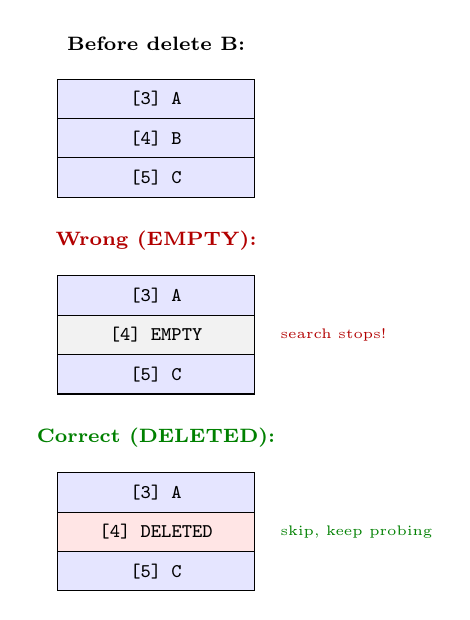
\begin{tikzpicture}[
    >=Stealth,
    slot/.style={draw, minimum width=2.5cm, minimum height=0.5cm,
                 font=\scriptsize\ttfamily}
  ]
  % Before delete
  \node[font=\scriptsize\bfseries] at (0, 0.7) {Before delete B:};
  \node[slot, fill=blue!10] (b3) at (0, 0) {[3] A};
  \node[slot, fill=blue!10] (b4) at (0, -0.5) {[4] B};
  \node[slot, fill=blue!10] (b5) at (0, -1.0) {[5] C};

  % After delete (wrong way)
  \node[font=\scriptsize\bfseries, text=red!70!black] at (0, -1.8) {Wrong (EMPTY):};
  \node[slot, fill=blue!10] (w3) at (0, -2.5) {[3] A};
  \node[slot, fill=gray!10] (w4) at (0, -3.0) {[4] EMPTY};
  \node[slot, fill=blue!10] (w5) at (0, -3.5) {[5] C};
  \node[font=\tiny, text=red!70!black, right=0.2cm of w4] {search stops!};

  % After delete (right way)
  \node[font=\scriptsize\bfseries, text=green!50!black] at (0, -4.3)
    {Correct (DELETED):};
  \node[slot, fill=blue!10] (c3) at (0, -5.0) {[3] A};
  \node[slot, fill=red!10] (c4) at (0, -5.5) {[4] DELETED};
  \node[slot, fill=blue!10] (c5) at (0, -6.0) {[5] C};
  \node[font=\tiny, text=green!50!black, right=0.2cm of c4] {skip, keep probing};
\end{tikzpicture}
\end{center}
\end{column}
\end{columns}
\end{frame}

% ===========================================================================
\section{Configuration}
% ===========================================================================

\begin{frame}[fragile]{Compile-Time Configuration}
\begin{columns}[T]
\begin{column}{0.48\textwidth}
\begin{lstlisting}[style=cstyle,
  title={Configurable parameters}]
/* Maximum table capacity */
#ifndef TIKU_KITS_DS_HTABLE_MAX_SIZE
#define TIKU_KITS_DS_HTABLE_MAX_SIZE 16
#endif
\end{lstlisting}

\vspace{0.3em}
\begin{block}{Load Factor Guidance}
\begin{itemize}
  \item Best: 50--70\% occupancy
  \item For 10 entries, use capacity 16
  \item High load $\Rightarrow$ more collisions $\Rightarrow$ slower
  \item Above 80\% performance degrades significantly
\end{itemize}
\end{block}
\end{column}

\begin{column}{0.48\textwidth}
\begin{lstlisting}[style=cstyle,
  title={Runtime initialization}]
struct tiku_kits_ds_htable ht;

/* 8 slots for ~5-6 entries */
tiku_kits_ds_htable_init(&ht, 8);

/* Or use maximum capacity */
tiku_kits_ds_htable_init(&ht,
    TIKU_KITS_DS_HTABLE_MAX_SIZE);
\end{lstlisting}

\vspace{0.3em}
\begin{table}
\centering
\scriptsize
\begin{tabular}{@{}rrrr@{}}
\toprule
\textbf{Capacity} & \textbf{Ideal Max} & \textbf{Load} & \textbf{RAM} \\
\midrule
4  & 3   & 75\%  & 40\,B \\
8  & 5   & 62\%  & 76\,B \\
16 & 11  & 69\%  & 148\,B \\
32 & 22  & 69\%  & 292\,B \\
\bottomrule
\end{tabular}
\end{table}
\end{column}
\end{columns}
\end{frame}

% ===========================================================================
\section{Implementation Details}
% ===========================================================================

\begin{frame}[fragile]{Put: Insert or Update}
\begin{lstlisting}[style=cstyle,
  title={tiku\_kits\_ds\_htable.c --- put (simplified)}]
int tiku_kits_ds_htable_put(struct tiku_kits_ds_htable *ht,
                             tiku_kits_ds_htable_key_t key,
                             tiku_kits_ds_elem_t value)
{
    uint16_t start = hash_fnv1a(key, ht->capacity);
    uint16_t idx = start;
    int found_deleted = 0;
    uint16_t first_deleted = 0;

    do {
        struct tiku_kits_ds_htable_entry *e = &ht->entries[idx];

        if (e->state == TIKU_KITS_DS_HTABLE_EMPTY) {
            /* Insert at first deleted slot or here */
            if (found_deleted) { idx = first_deleted; e = &ht->entries[idx]; }
            e->key = key;  e->value = value;
            e->state = TIKU_KITS_DS_HTABLE_OCCUPIED;
            ht->count++;
            return TIKU_KITS_DS_OK;
        }
        if (e->state == TIKU_KITS_DS_HTABLE_DELETED && !found_deleted) {
            found_deleted = 1;  first_deleted = idx;
        } else if (e->key == key) {
            e->value = value;   /* update in place */
            return TIKU_KITS_DS_OK;
        }
        idx = (idx + 1) % ht->capacity;
    } while (idx != start);

    return TIKU_KITS_DS_ERR_FULL;
}
\end{lstlisting}
\end{frame}

% ---------------------------------------------------------------------------
\begin{frame}[fragile]{Get and Remove}
\begin{columns}[T]
\begin{column}{0.48\textwidth}
\begin{lstlisting}[style=cstyle,
  title={get --- linear probe lookup}]
int tiku_kits_ds_htable_get(
    const struct tiku_kits_ds_htable *ht,
    tiku_kits_ds_htable_key_t key,
    tiku_kits_ds_elem_t *value)
{
    uint16_t start, idx;
    start = hash_fnv1a(key,
                       ht->capacity);
    idx = start;

    do {
        const struct
            tiku_kits_ds_htable_entry *e
            = &ht->entries[idx];

        if (e->state ==
            TIKU_KITS_DS_HTABLE_EMPTY)
            return
              TIKU_KITS_DS_ERR_NOTFOUND;

        if (e->state ==
            TIKU_KITS_DS_HTABLE_OCCUPIED
            && e->key == key) {
            *value = e->value;
            return TIKU_KITS_DS_OK;
        }
        idx = (idx + 1) % ht->capacity;
    } while (idx != start);

    return TIKU_KITS_DS_ERR_NOTFOUND;
}
\end{lstlisting}
\end{column}

\begin{column}{0.48\textwidth}
\begin{lstlisting}[style=cstyle,
  title={remove --- tombstone deletion}]
int tiku_kits_ds_htable_remove(
    struct tiku_kits_ds_htable *ht,
    tiku_kits_ds_htable_key_t key)
{
    uint16_t start, idx;
    start = hash_fnv1a(key,
                       ht->capacity);
    idx = start;

    do {
        struct
            tiku_kits_ds_htable_entry *e
            = &ht->entries[idx];

        if (e->state ==
            TIKU_KITS_DS_HTABLE_EMPTY)
            return
              TIKU_KITS_DS_ERR_NOTFOUND;

        if (e->state ==
            TIKU_KITS_DS_HTABLE_OCCUPIED
            && e->key == key) {
            e->state =
              TIKU_KITS_DS_HTABLE_DELETED;
            ht->count--;
            return TIKU_KITS_DS_OK;
        }
        idx = (idx + 1) % ht->capacity;
    } while (idx != start);

    return TIKU_KITS_DS_ERR_NOTFOUND;
}
\end{lstlisting}
\end{column}
\end{columns}
\end{frame}

% ===========================================================================
\section{Examples}
% ===========================================================================

\begin{frame}[fragile]{Example 1: FRAM Key-Value Configuration Store}
\begin{lstlisting}[style=cstyle,
  title={Persistent configuration with key-value lookup}]
#define CFG_SAMPLE_RATE  0x0001
#define CFG_TX_POWER     0x0002
#define CFG_SENSOR_MASK  0x0003
#define CFG_ALARM_THRESH 0x0004

struct tiku_kits_ds_htable config;
tiku_kits_ds_elem_t val;

tiku_kits_ds_htable_init(&config, 8);

/* Store configuration parameters */
tiku_kits_ds_htable_put(&config, CFG_SAMPLE_RATE, 500);   /* 500 ms */
tiku_kits_ds_htable_put(&config, CFG_TX_POWER, 3);        /* dBm */
tiku_kits_ds_htable_put(&config, CFG_SENSOR_MASK, 0x0F);  /* 4 sensors */
tiku_kits_ds_htable_put(&config, CFG_ALARM_THRESH, 85);   /* degrees */

/* Lookup a config value --- O(1) average */
if (tiku_kits_ds_htable_get(&config, CFG_TX_POWER, &val)
    == TIKU_KITS_DS_OK) {
    set_radio_power((int8_t)val);
}

/* Update a parameter in place */
tiku_kits_ds_htable_put(&config, CFG_SAMPLE_RATE, 1000);  /* slower rate */
\end{lstlisting}
\end{frame}

% ---------------------------------------------------------------------------
\begin{frame}[fragile]{Example 2: Device Address Registry}
\begin{columns}[T]
\begin{column}{0.52\textwidth}
\begin{lstlisting}[style=cstyle,
  title={Map I2C addresses to driver IDs}]
#define DRV_TEMP     1
#define DRV_ACCEL    2
#define DRV_HUMIDITY 3

struct tiku_kits_ds_htable dev_map;
tiku_kits_ds_elem_t driver_id;

tiku_kits_ds_htable_init(&dev_map, 8);

/* Register devices by I2C address */
tiku_kits_ds_htable_put(
    &dev_map, 0x48, DRV_TEMP);
tiku_kits_ds_htable_put(
    &dev_map, 0x1D, DRV_ACCEL);
tiku_kits_ds_htable_put(
    &dev_map, 0x40, DRV_HUMIDITY);

/* Lookup driver for address */
uint32_t addr = read_i2c_address();
if (tiku_kits_ds_htable_get(
        &dev_map, addr, &driver_id)
    == TIKU_KITS_DS_OK) {
    dispatch_to_driver(
        (uint8_t)driver_id);
}
\end{lstlisting}
\end{column}

\begin{column}{0.44\textwidth}
\begin{center}
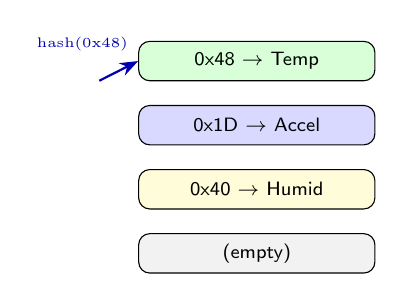
\begin{tikzpicture}[
    >=Stealth,
    entry/.style={draw, rounded corners, minimum width=3cm,
                  minimum height=0.5cm, font=\scriptsize\sffamily}
  ]
  \node[entry, fill=green!15] (e1) {0x48 $\rightarrow$ Temp};
  \node[entry, fill=blue!15, below=0.3cm of e1] (e2) {0x1D $\rightarrow$ Accel};
  \node[entry, fill=yellow!15, below=0.3cm of e2] (e3) {0x40 $\rightarrow$ Humid};
  \node[entry, fill=gray!10, below=0.3cm of e3] (e4) {(empty)};

  \draw[->, thick, blue!70!black] (-2.0, -0.25) -- (e1.west)
    node[above left, font=\tiny] {hash(0x48)};
\end{tikzpicture}
\end{center}

\vspace{0.5em}
\begin{block}{Fast Device Dispatch}
When an interrupt arrives from an I2C address,
look up the driver in $O(1)$ average time.
No linear scan through an array of device structs.
\end{block}
\end{column}
\end{columns}
\end{frame}

% ---------------------------------------------------------------------------
\begin{frame}[fragile]{Example 3: Collision and Re-insertion}
\begin{lstlisting}[style=cstyle,
  title={Demonstrating collision handling and tombstone reuse}]
struct tiku_kits_ds_htable ht;
tiku_kits_ds_elem_t val;

/* Small capacity to force collisions */
tiku_kits_ds_htable_init(&ht, 4);

/* Insert 4 keys --- guaranteed collisions with capacity=4 */
tiku_kits_ds_htable_put(&ht, 1,  10);
tiku_kits_ds_htable_put(&ht, 5,  50);
tiku_kits_ds_htable_put(&ht, 9,  90);
tiku_kits_ds_htable_put(&ht, 13, 130);

/* Remove key=5 (creates tombstone) */
tiku_kits_ds_htable_remove(&ht, 5);

/* Key=9 still findable --- tombstone does NOT break probe chain */
tiku_kits_ds_htable_get(&ht, 9, &val);    /* val == 90 */

/* Re-insert at tombstone slot */
tiku_kits_ds_htable_put(&ht, 5, 999);
tiku_kits_ds_htable_get(&ht, 5, &val);    /* val == 999 */
\end{lstlisting}
\end{frame}

% ===========================================================================
\section{Test Suite}
% ===========================================================================

\begin{frame}{Test Cases Overview}
\begin{table}
\centering
\small
\begin{tabular}{@{}clp{7cm}@{}}
\toprule
\textbf{\#} & \textbf{Test Function} & \textbf{What It Verifies} \\
\midrule
1 & \texttt{test\_kits\_ds\_htable\_init}
  & Initialization, parameter validation, entries EMPTY \\
2 & \texttt{test\_kits\_ds\_htable\_put\_get}
  & Insert 3 pairs, retrieve all, miss returns NOTFOUND \\
3 & \texttt{test\_kits\_ds\_htable\_update\_existing}
  & Put same key twice updates value, count stays 1 \\
4 & \texttt{test\_kits\_ds\_htable\_remove\_tombstone}
  & Remove creates tombstone, other keys intact, re-insert \\
5 & \texttt{test\_kits\_ds\_htable\_contains}
  & Contains returns 1/0 correctly, works after remove \\
6 & \texttt{test\_kits\_ds\_htable\_collision\_handling}
  & Forced collisions with cap=4, tombstone probe chains \\
7 & \texttt{test\_kits\_ds\_htable\_full\_table}
  & ERR\_FULL on overflow, update in full table OK \\
8 & \texttt{test\_kits\_ds\_htable\_clear\_reset}
  & Clear marks all EMPTY, table reusable \\
9 & \texttt{test\_kits\_ds\_htable\_null\_inputs}
  & All functions reject NULL with ERR\_NULL \\
\bottomrule
\end{tabular}
\end{table}
\end{frame}

% ===========================================================================
\section{Summary}
% ===========================================================================

\begin{frame}{Summary}
\begin{columns}[T]
\begin{column}{0.48\textwidth}
\begin{block}{What We Built}
\begin{itemize}
  \item Open-addressed hash table
  \item FNV-1a hash for uint32\_t keys
  \item Linear probing for collision resolution
  \item Tombstone deletion preserves probe chains
  \item 148 bytes RAM (default cap=16), no heap
\end{itemize}
\end{block}

\begin{block}{Key Design Choices}
\begin{itemize}
  \item Three-state slots (EMPTY/OCCUPIED/DELETED)
  \item Upsert semantics for \texttt{put()}
  \item Tombstone reuse on insertion
  \item Size to $\sim$70\% load factor
\end{itemize}
\end{block}
\end{column}

\begin{column}{0.48\textwidth}
\begin{block}{Use Cases}
\begin{itemize}
  \item FRAM key-value configuration store
  \item Device address to driver mapping
  \item Command/string-to-enum lookup
  \item Sensor ID registry
\end{itemize}
\end{block}

\begin{block}{Files}
\scriptsize
\begin{tabular}{@{}lp{4.5cm}@{}}
Header: & \texttt{ds/htable/tiku\_kits\_ds\_htable.h} \\
Source: & \texttt{ds/htable/tiku\_kits\_ds\_htable.c} \\
Tests: & \texttt{tests/ds/test\_kits\_ds\_htable.c} \\
Common: & \texttt{ds/tiku\_kits\_ds.h} \\
\end{tabular}
\end{block}
\end{column}
\end{columns}
\end{frame}

% ---------------------------------------------------------------------------
\begin{frame}{Thank You}
\begin{center}
\Large\textbf{TikuKits DS: Hash Table}\\[0.5em]
\normalsize Constant-Time Key-Value Lookup for Physical AI Endpoints\\[1.5em]

\begin{tabular}{rl}
  Repository: & \url{https://github.com/tikuos/tikuOS} \\
  License:    & Apache 2.0 \\
  Common:     & \texttt{tikukits/ds/tiku\_kits\_ds.h} \\
  Header:     & \texttt{tikukits/ds/htable/tiku\_kits\_ds\_htable.h} \\
  Source:     & \texttt{tikukits/ds/htable/tiku\_kits\_ds\_htable.c} \\
  Tests:      & \texttt{tikukits/tests/ds/test\_kits\_ds\_htable.c} \\
\end{tabular}
\end{center}
\end{frame}

\end{document}
